\documentclass[11pt, oneside]{article}
\usepackage{geometry}
\usepackage{animate}
\usepackage{graphicx}
\usepackage{amssymb}
\usepackage{amsmath}
\usepackage[
  backend=bibtex,
  style=numeric,
  sorting=none,
  citestyle=numeric-comp
]{biblatex}
\addbibresource{references.bib}

\geometry{letterpaper}

\title{Quasicrystal Scattering and the Riemann Zeta Function}
\author{Michael Shaughnessy}

\begin{document}
\maketitle

\begin{abstract}
I carry out numerical scattering calculations against a family of finite-length one-dimensional point-like arrangements of atoms, $\chi(x)$, related to the distribution of prime numbers by a shift operation making the atomic density approximately constant. 
I show how the Riemann Zeta Function (RZF) naturally parameterizes the analytic structure of the scattering amplitude and give numerical results.
\end{abstract}

\section{Introduction}

There have been many explanations of the curious relationship between the prime numbers and the values of the non-trivial zeros of the Riemann Zeta Function (RZF) \cite{Riemann1859, Selberg1956, Dyson2009, Zhang2014}.

Freeman Dyson \cite{Baez2013} speculated about a possible path to determining the relationship between the real and the imaginary components of the non-trivial zeros of the RZF, using the concept of a quasicrystal.

A quasiperiodic crystal, or quasicrystal, is a structure that is ordered but not periodic. Quasicrystals were experimentally observed by Shechtman in 1984 \cite{Shectman1984}. 

B. Riemann showed the prime numbers are partially ordered and are not periodic \cite{Riemann1859} in 1859, and H. von Mangoldt \cite{VonMangoldt1895} proved the explicit formula in 1895.

The explicit formula of Guinand and Weil \cite{Weil} is a formula for the Fourier transform of the RZF zeros as a sum over prime powers, plus additional terms.  

\begin{equation}
\sum_{\rho} h(\rho) = h(0) + h(1) - \sum_{p} \sum_{m=1}^{\infty} \frac{h(\log p^m)}{p^{m/2}} \log p - \int_{-\infty}^{\infty} \frac{h(t) \Phi(t)}{2} dt
\end{equation}

The explicit formula of Guinand and Weil is the dual of the prime counting function expression of von Mangoldt \cite{VonMangoldt1895}.

\subsection{Fourier Transform}
The Fourier transform of $V(x)$ is $\hat{V}(k)$:

\begin{equation}
\hat{V}(k) = \int_{-\infty}^{\infty}V(x)e^{-i2\pi kx}dx
\end{equation}

The physical process of scattering a wave from a potential can be represented by applying the Fourier transform to the potential. The result is a function on the space of wave momentum (reciprocal or dual space), often called the spectrum or scattering amplitude of the wave against the potential. The scattering amplitude can be measured by plotting the number of times a reflected wave arrives back at the wave source as a function of the wave momentum, $k$.

A one-dimensional scattering potential may be of the form:
\begin{equation}
V(x) = \sum_{x_n \in X}\delta(x - x_n)
\end{equation} 
 
where the $x_n$ are elements of a countable set of real numbers, and $\delta(x)$ is the Dirac delta function. Then $V(x)$ is called a tempered distribution.

For certain $V(x)$ of the form above, it is the case that its Fourier transform, $\hat{V}(k)$, also contains a tempered distribution:
  
\begin{equation}
 \label{eq: RiemannFourier}
 \mathcal{F}\left \{V(x)\right \} = \hat{V}(k) = \mathcal{F}\left \{ \sum_{x_n \in X}\delta(x - x_n) \right \} = \hat{h}(k) +  \sum_{k_m \in X^{*}} \hat{V}_{m} \delta(k - k_{m})
\end{equation}

Here, $X^*$ denotes the dual set of $X$, $\hat{V}_{m}$ are coefficients, and $\hat{h}(k)$ is a continuous function.

If $\hat{h}(k) = 0$ everywhere, then $V(x)$ is called a quasicrystal.

By applying the Fourier transform a second time to $\hat{V}(k)$, it is evident that $\hat{V}(k)$ is also a quasicrystal when $V(x)$ is a quasicrystal. When all the $x_n$ lie along a line, the $k_m$ must also lie along a line in the complex plane—applying the Fourier transform twice gives us back our original $V(x)$.

\subsection{Wave Scattering and $\chi$}
Inspired by Varma's approach \cite{Varma2016}, I define a specific 1-dimensional arrangement of atoms suitable for scattering calculations through a normalization or shift operation yielding an approximately constant atomic density.

I apply the shift transformation directly to the real-space atomic positions, as opposed to the k-space positions of the zeros of the RZF in \cite{Varma2016}.

Consider a scattering potential, $V(x)$, which is a distribution of Dirac delta functions along the positive real line, one at each prime number.

The delta functions are located at integers and so they have spacing at least 1. They do not have a maximum spacing \cite{Westzynthius1931, Erdos1950}.

The exact expression \cite{Riemann1859} for $\pi(x)$ when $x>1$ is:

\begin{equation}
\pi(x) = \pi_0(x) - \frac{1}{2} = R(x) - \sum_{\rho}R(x^{\rho}) - \frac{1}{2}
\end{equation}

where

\begin{equation}
R(x) = \sum_{n=1}^{\infty}\frac{\mu(n)}{n}\operatorname{li}(x^{\frac{1}{n}})
\end{equation}

Here, $\mu(n)$ is the Möbius function, $\operatorname{li}(x)$ is the logarithmic integral function, and $\rho$ runs over all the zeros of the RZF.

If the trivial zeros are collected and the sum is taken only over the non-trivial zeros, then:

\begin{equation}
\pi_0(x) \approx R(x) - \sum_{\rho}R(x^{\rho}) - \frac{1}{\log(x)} + \frac{1}{\pi}\arctan\left(\frac{1}{\log(x)}\right)
\end{equation}
 
It is well known that $\pi(x) \sim \frac{x}{\log(x)}$ in a rougher approximation.

The quantity $\frac{\pi(x)}{x}$ has units of density—it represents the density of atoms around $x$ in the scattering potential defined by $V(x)$.

In the numerical calculations below, I normalize the positions of the atoms in $V(x)$ with a shift operation, such that the density of atoms becomes approximately constant, yielding a shifted tempered distribution with finite spacing and asymptotically constant density. Call this potential $\chi(x)$ and define the shift operator $p$:

\begin{equation}
p(x_n) = x_n \cdot \frac{1}{\pi(x_n)} \approx \log(x_n)
\end{equation}

where $x_n$ is the $n$th prime number and $\pi(x_n)$ is the prime counting function.

The shift operation applied to the atomic positions serves to normalize the density of atoms in the potential $V(x)$. Since the primes become sparser as numbers increase, the raw potential with delta functions at prime positions has a decreasing density. By applying the shift $p(x_n) = x_n \cdot \frac{1}{\pi(x_n)}$, we effectively map the positions such that the density becomes approximately constant. This is because $\pi(x_n)$, the prime counting function, counts the number of primes less than or equal to $x_n$, and therefore $x_n / \pi(x_n)$ gives an average spacing between primes up to $x_n$. Since $\pi(x) \sim x / \log x$, we have $x_n / \pi(x_n) \approx \log x_n$. Thus, the shift operation maps the primes to positions approximately proportional to $\log x_n$.

This shift is significant because the logarithmic behavior is connected to the zeros of the RZF through the explicit formulae in analytic number theory. When we consider the Fourier transform of the shifted potential $\chi(x)$, the zeros of the RZF manifest themselves in the scattering amplitude due to the oscillatory terms arising from the non-trivial zeros in the explicit formula for $\pi(x)$. Specifically, the RZF zeros influence the distribution of primes and therefore affect the structure of $\chi(x)$, leading to features in the scattering amplitude at positions corresponding to the imaginary parts of the RZF zeros.

I carry out numerical scattering calculations on finite-length approximations (parameterized by the total number of atoms, $L_{\chi}$) of the potential $\chi(x)$.

\begin{figure}[htbp]
\begin{center}
    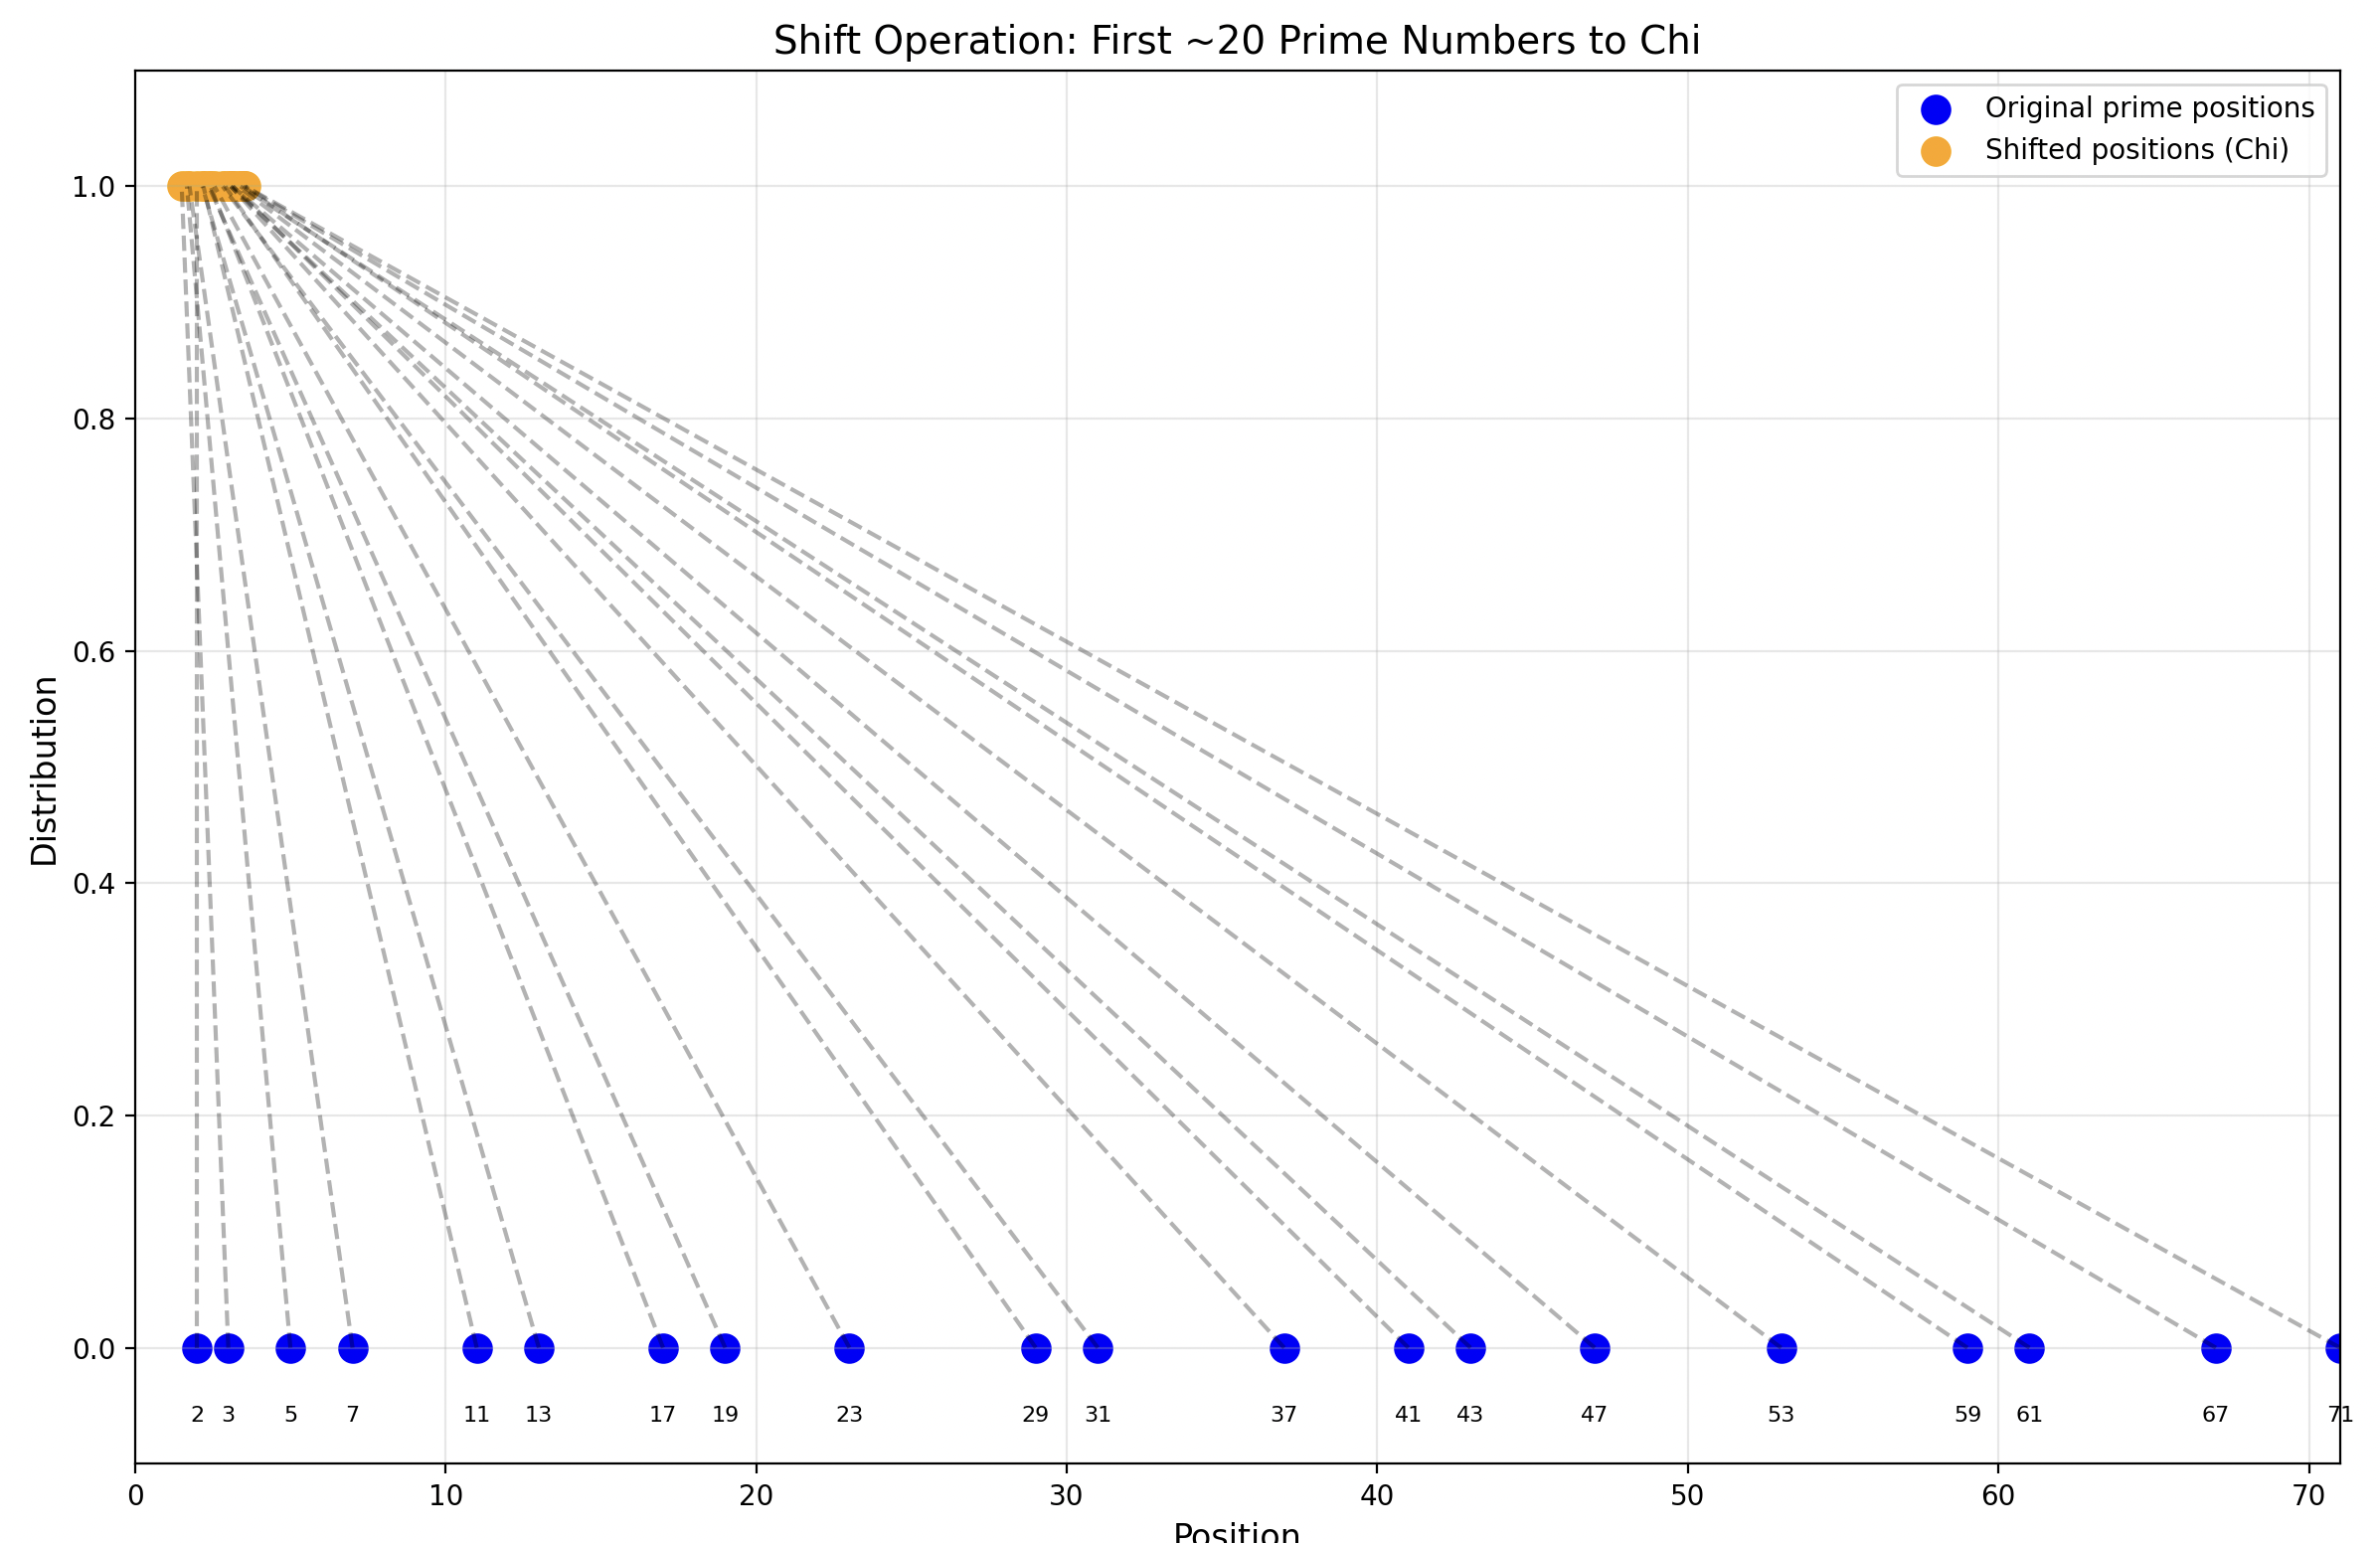
\includegraphics[width=0.8\linewidth]{normalizing.png}
\caption{Normalized atomic positions in the $\chi(x)$ potential. The x-axis represents the index of each atom, while the y-axis shows its normalized position.}
\label{fig:normalized_positions}
\end{center}
\end{figure}

Figure \ref{fig:normalized_positions} shows the normalized positions of atoms in our $\chi(x)$ potential. This normalization is crucial for understanding how the RZF zeros enter our scattering calculation.

This connection explains the correspondence we observe between the peaks in our scattering amplitude and the positions of the RZF zeros. Each zero contributes to the scattering process through these poles, manifesting as features in the scattering spectrum.

This relationship not only provides insight into the mathematical structure of our scattering problem but also offers a physical interpretation of the RZF zeros in terms of wave scattering from a carefully constructed potential. Further exploration of the properties of the RZF and its zeros through the lens of physical scattering processes could be beneficial.

\section{Results}
\begin{figure}[htbp]
\begin{center}
    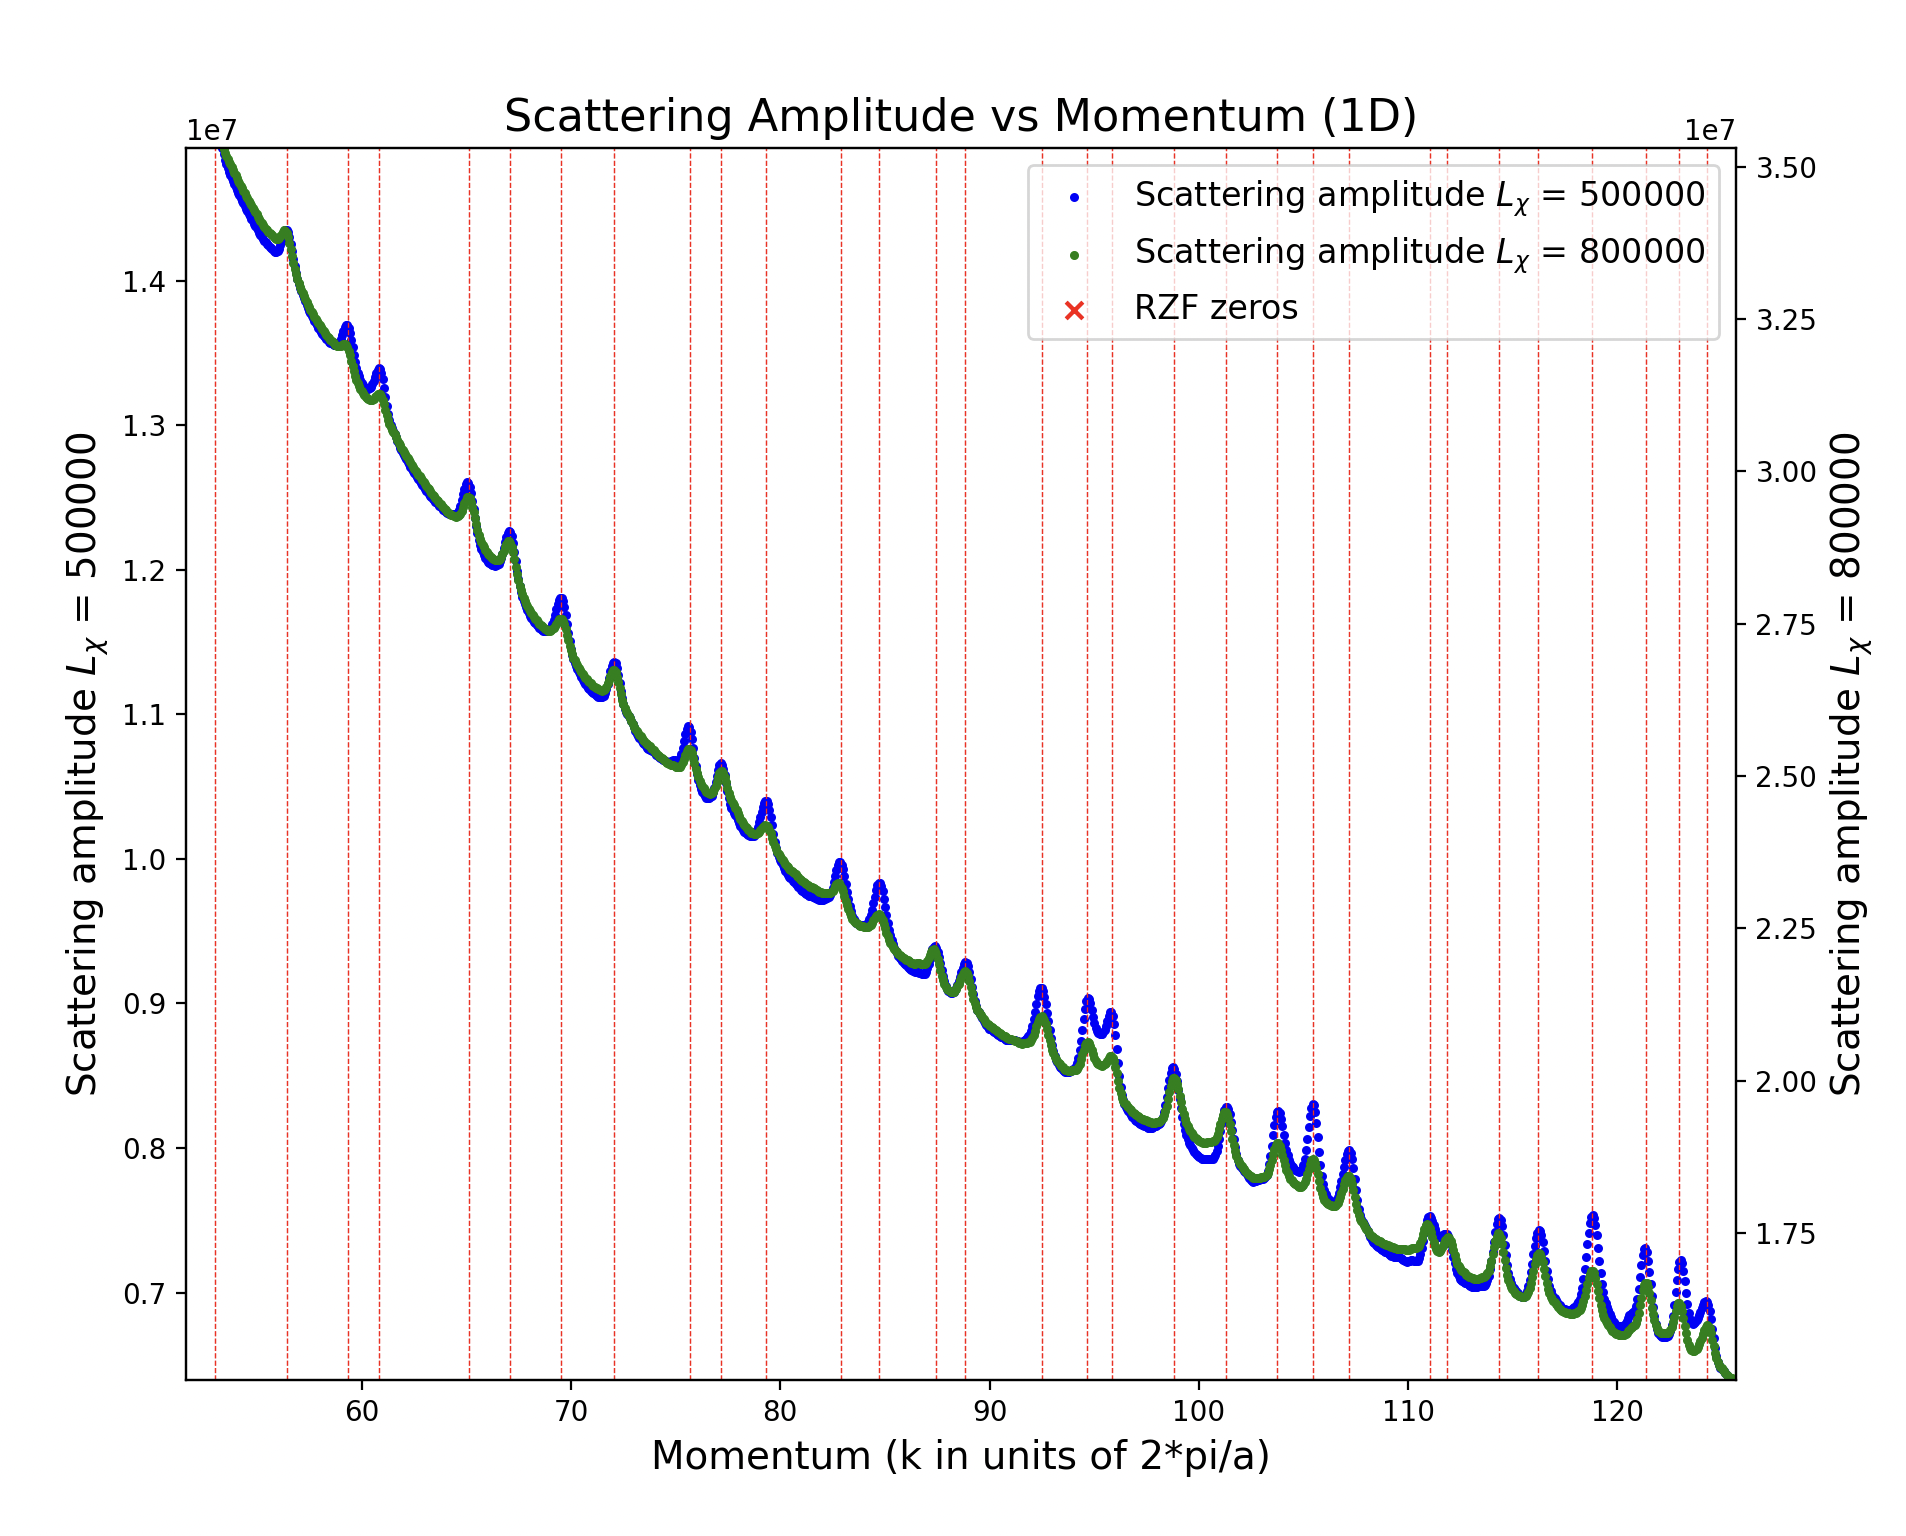
\includegraphics[width=0.8\linewidth]{zoomed_scattering.png}
\caption{Scattering amplitude for finite $L_{\chi}$. Vertical red lines indicate the positions of the imaginary part of the non-trivial zeros of the RZF.}
\label{fig:scattering_amplitude}
\end{center}
\end{figure}

\section{Method}

Code for the scattering calculation is available at:
 
\url{https://github.com/mickeyshaughnessy/quasicrystal/blob/main/scattering.py}
 
\begin{figure}[htbp]
\begin{center}
    %\includegraphics[width=0.8\linewidth]{../images/scattering_code.png}
    \includegraphics[width=0.8\linewidth]{scattering_code.png}
\caption{Code for computing scattering amplitude}
\label{fig:scattering_code}
\end{center}
\end{figure}
 
\begin{figure}[htbp]
\begin{center}
    %\includegraphics[width=0.8\linewidth]{../images/plotting_code.png}
     \includegraphics[width=0.8\linewidth]{plotting_code.png}

\caption{Code for generating spectral plot}
\label{fig:plotting_code}
\end{center}
\end{figure}

\subsection{Analytical Computation}

In this section, we compute the Fourier transform of the shifted potential $\chi(x)$ and demonstrate how the non-trivial zeros of the Riemann Zeta Function (RZF) contribute to the scattering amplitude.

Recall that the shifted potential is given by:

\begin{equation}
\chi(x) = \sum_{p \in P} \delta\left(x - \log p\right),
\end{equation}

where $P$ is the set of prime numbers, and $\delta(x)$ is the Dirac delta function. The shift operation effectively maps each prime $p$ to $x = \log p$, resulting in an approximately constant density of atomic positions.

The Fourier transform of $\chi(x)$ is:

\begin{equation}
\hat{\chi}(k) = \int_{-\infty}^{\infty} \chi(x) e^{-i 2\pi k x} dx = \sum_{p \in P} e^{-i 2\pi k \log p} = \sum_{p \in P} p^{-i 2\pi k}.
\end{equation}

Our goal is to analyze the analytic structure of $\hat{\chi}(k)$ and understand how the zeros of the RZF contribute to the scattering amplitude.

\subsubsection{Connection to the Riemann Zeta Function}

The expression $\hat{\chi}(k) = \sum_{p} p^{-i 2\pi k}$ involves a sum over primes raised to a complex exponent. To relate this sum to the RZF, we consider the logarithmic derivative of the RZF, which is intimately connected to prime numbers through its Euler product representation.

The RZF is defined for $\operatorname{Re}(s) > 1$ by:

\begin{equation}
\zeta(s) = \prod_{p \in P} \frac{1}{1 - p^{-s}}.
\end{equation}

Taking the natural logarithm of both sides, we obtain:

\begin{equation}
\log \zeta(s) = -\sum_{p \in P} \log\left(1 - p^{-s}\right) = \sum_{p \in P} \sum_{m=1}^\infty \frac{1}{m} p^{-m s},
\end{equation}

where we have expanded the logarithm using the Taylor series for $\log(1 - x)$ valid for $|x| < 1$.

Differentiating both sides with respect to $s$, we obtain the logarithmic derivative:

\begin{equation}
\frac{\zeta'(s)}{\zeta(s)} = -\sum_{p \in P} \sum_{m=1}^\infty \log p \cdot p^{-m s}.
\end{equation}

This expression highlights that the poles of $\frac{\zeta'(s)}{\zeta(s)}$ occur at the zeros of $\zeta(s)$. The sum over $m$ accounts for all powers of primes, but our Fourier transform involves only the first power ($m = 1$). To connect our sum to the logarithmic derivative, we consider the von Mangoldt function $\Lambda(n)$:

\begin{equation}
\Lambda(n) = \begin{cases}
\log p & \text{if } n = p^m \text{ for some prime } p \text{ and integer } m \geq 1, \\
0 & \text{otherwise}.
\end{cases}
\end{equation}

Using $\Lambda(n)$, we can write:

\begin{equation}
-\frac{\zeta'(s)}{\zeta(s)} = \sum_{n=1}^\infty \Lambda(n) n^{-s}.
\end{equation}

Our Fourier transform resembles this expression but lacks the $\Lambda(n)$ factor. However, we can consider a modified sum where we divide by $\log n$:

\begin{equation}
\sum_{n=2}^\infty \frac{\Lambda(n)}{\log n} n^{-s} = \sum_{p \in P} p^{-s} + \sum_{p \in P} \sum_{m=2}^\infty \frac{\log p}{\log p^m} p^{-m s}.
\end{equation}

For $m = 1$, we have $\frac{\log p}{\log p} = 1$, and the term simplifies to $p^{-s}$, matching the terms in our Fourier transform $\hat{\chi}(k)$. This suggests that our sum is related to the logarithmic derivative of the RZF.

\subsubsection{Application of the Residue Theorem}

To further elucidate the connection, we consider an integral representation of our sum and apply the residue theorem. We define the function:

\begin{equation}
S(k) = \sum_{p \in P} p^{-i 2\pi k}.
\end{equation}

Since the sum diverges for real $k$, we introduce a convergence factor $p^{-\epsilon}$ with $\epsilon > 0$, allowing us to write a convergent sum:

\begin{equation}
S_\epsilon(k) = \sum_{p \in P} p^{- \epsilon - i 2\pi k}.
\end{equation}

We can express $S_\epsilon(k)$ as a complex integral involving the logarithmic derivative of the RZF:

\begin{equation}
S_\epsilon(k) = \frac{1}{2\pi i} \int_{c - i \infty}^{c + i \infty} -\frac{\zeta'(s)}{\zeta(s)} \cdot \frac{1}{s - (\epsilon + i 2\pi k)} ds,
\end{equation}

where $c > 1$ ensures the integral converges.

The integrand has simple poles at $s = \rho$, the non-trivial zeros of the RZF, and at $s = \epsilon + i 2\pi k$ due to the term $\frac{1}{s - (\epsilon + i 2\pi k)}$.

Applying the residue theorem, the integral evaluates to:

\begin{equation}
S_\epsilon(k) = \sum_{\rho} \frac{1}{\rho - (\epsilon + i 2\pi k)} + \frac{\zeta'(\epsilon + i 2\pi k)}{\zeta(\epsilon + i 2\pi k)}.
\end{equation}

As $\epsilon \to 0$, the term $\frac{\zeta'(\epsilon + i 2\pi k)}{\zeta(\epsilon + i 2\pi k)}$ may have poles if $\epsilon + i 2\pi k$ coincides with a zero of $\zeta(s)$. The poles at the zeros $\rho$ of $\zeta(s)$ contribute terms of the form:

\begin{equation}
\operatorname{Res}\left(-\frac{\zeta'(s)}{\zeta(s)}, s = \rho\right) \cdot \frac{1}{\rho - i 2\pi k} = \frac{1}{\rho - i 2\pi k}.
\end{equation}

Thus, the sum over the residues at the zeros of the RZF manifests in the scattering amplitude:

\begin{equation}
S(k) = \lim_{\epsilon \to 0} S_\epsilon(k) = \sum_{\rho} \frac{1}{\rho - i 2\pi k} + \frac{\zeta'(i 2\pi k)}{\zeta(i 2\pi k)}.
\end{equation}

The term $\frac{\zeta'(i 2\pi k)}{\zeta(i 2\pi k)}$ reflects the contribution from the pole at $s = i 2\pi k$.

These terms highlight the direct contribution of the RZF zeros to the Fourier transform $\hat{\chi}(k)$.

\subsubsection{Interpretation of the Scattering Amplitude}

The presence of poles at $s = \rho$ in the integral representation of $S(k)$ implies that the non-trivial zeros of the RZF contribute significantly to the scattering amplitude. Specifically, the scattering amplitude $\hat{\chi}(k)$ exhibits resonances at values of $k$ corresponding to the imaginary parts of the RZF zeros divided by $2\pi$.

These resonances are reflected as peaks in the scattering amplitude, as observed in our numerical results. The correspondence between the peaks in $\hat{\chi}(k)$ and the RZF zeros arises because the poles in the complex plane contribute to the integral via the residue theorem, amplifying the scattering amplitude at those specific $k$ values.

\subsubsection{Summary of the Analytical Connection}

In summary, the zeros of the RZF enter our scattering calculation through the analytic structure of the Fourier transform of $\chi(x)$. The shifted positions of the primes lead to an expression for $\hat{\chi}(k)$ involving the sum $\sum_{p} p^{-i 2\pi k}$, which is intimately connected to the logarithmic derivative of the RZF.

By introducing a convergence factor and applying complex analysis techniques, we demonstrate that the non-trivial zeros of the RZF contribute poles to the scattering amplitude. These poles correspond to resonances in the scattering process, and their positions align with the imaginary parts of the non-trivial zeros of the RZF divided by $2\pi$.

This analytical computation explains the correspondence observed between the peaks in the scattering amplitude and the RZF zeros in our numerical results, providing a deep connection between number theory and wave scattering phenomena.


\section{Conclusion}

The results of our calculations, as presented in Figure \ref{fig:scattering_amplitude}, reveal:

1. The scattering amplitude exhibits a series of peaks and troughs, with the overall amplitude decreasing as momentum increases.

2. There is a clear correspondence between the positions of the RZF zeros and peaks in the scattering amplitude. Many of the prominent peaks in the scattering amplitude align closely with the RZF zeros.

3. The scattering amplitudes for different $L_\chi$ values show very similar behavior, suggesting that the observed features are robust and not artifacts of the finite lattice size.

4. The overall structure of the scattering amplitude, when viewed across a wider range of momentum values, shows a consistent pattern of peaks and troughs that seems to be related to the distribution of RZF zeros.

These observations support our physical picture of how the RZF zeros enter the scattering calculation through the normalization process. The peaks in the scattering amplitude that align with the RZF zeros are likely manifestations of the poles created by these zeros in the complex plane.

This work provides a novel physical interpretation of the RZF zeros in terms of wave scattering from a carefully constructed potential. It suggests that the RZF zeros might be understood as resonances in this scattering system, where each zero corresponds to a particular scattering mode.

Furthermore, the robustness of these features across different $L_\chi$ values suggests that this relationship between the RZF zeros and scattering amplitudes is not an artifact of our finite approximation, but rather a fundamental property of the system we've constructed.

Future work could explore extending this approach to higher dimensions, investigating the effects of different normalization schemes, or studying how perturbations to the potential affect the relationship between scattering amplitudes and RZF zeros.

In conclusion, this work demonstrates an intriguing connection between number theory, specifically the Riemann Zeta Function and its zeros, and the physics of wave scattering. It provides a new perspective on these mathematical objects and suggests potential new approaches for studying them through physical analogies.

\section{Acknowledgements}
I gratefully acknowledge helpful conversations with C.Y. Fong, John Baez, Jamison Galloway, Robert Hayre, Chun Yen Lin, Charles Martin, and Catalin Spataru.

\printbibliography

\end{document}
